%=======================+=========================
%================  Reconstruction  ================
%=================================================


\section[Event reconstruction]{Event reconstruction \label{sec:reconstruction}}

% Copy from GlueX-doc-3108
% "Production and Analysis of GlueX Data"
% TODO: UPDATE for 2017

During and after the experimental running, GlueX uses the computer center batch farm at Jefferson Lab to perform data monitoring, event reconstruction, and physics analyses.  For data monitoring, we study the detector hit occupancies, calibration and reconstruction quality, and experimental yields and resolutions for several physics channels.  We monitor a subset of the data as soon as it is saved to tape, submitting batch farm jobs via cron jobs.  Every few weeks, we perform monitoring launches on a subset of the data to study improvements from ongoing calibrations and reconstruction software improvements.  The histograms produced by these monitoring jobs are displayed on a web site and ROOT files are available for download, enabling the collaborators to easily study the quality of the data. 

Every few months we perform a major reconstruction launch over all of the data, linking the hits in the various detector systems to reconstruct particles in the physics events.  Monitoring plots from these launches are also published to the web. Finally, we regularly perform analysis launches over the reconstructed data, where a JANA plugin is used to filter out reactions that were previously specified by users in a web form. The results of these launches are saved in reaction-specific ROOT TTrees for further analysis.

For all launches, JANA was is multithreaded to make efficient use of the available computing resources. Figure~\ref{fig:offline_monitorA} shows the multithreaded scaling from our monitoring launches is near the theoretical limit.  
%SWIF is used to manage the batch farm jobs, and is queried to study the performance of the launches.  Figure~\ref{fig:farm-time} shows how many batch farm jobs were in each processing state as function of time our latest reconstruction launch.
All file outputs are written to a write-through cache system, which is ultimately backed up to tape.

\begin{figure}[h!]\centering
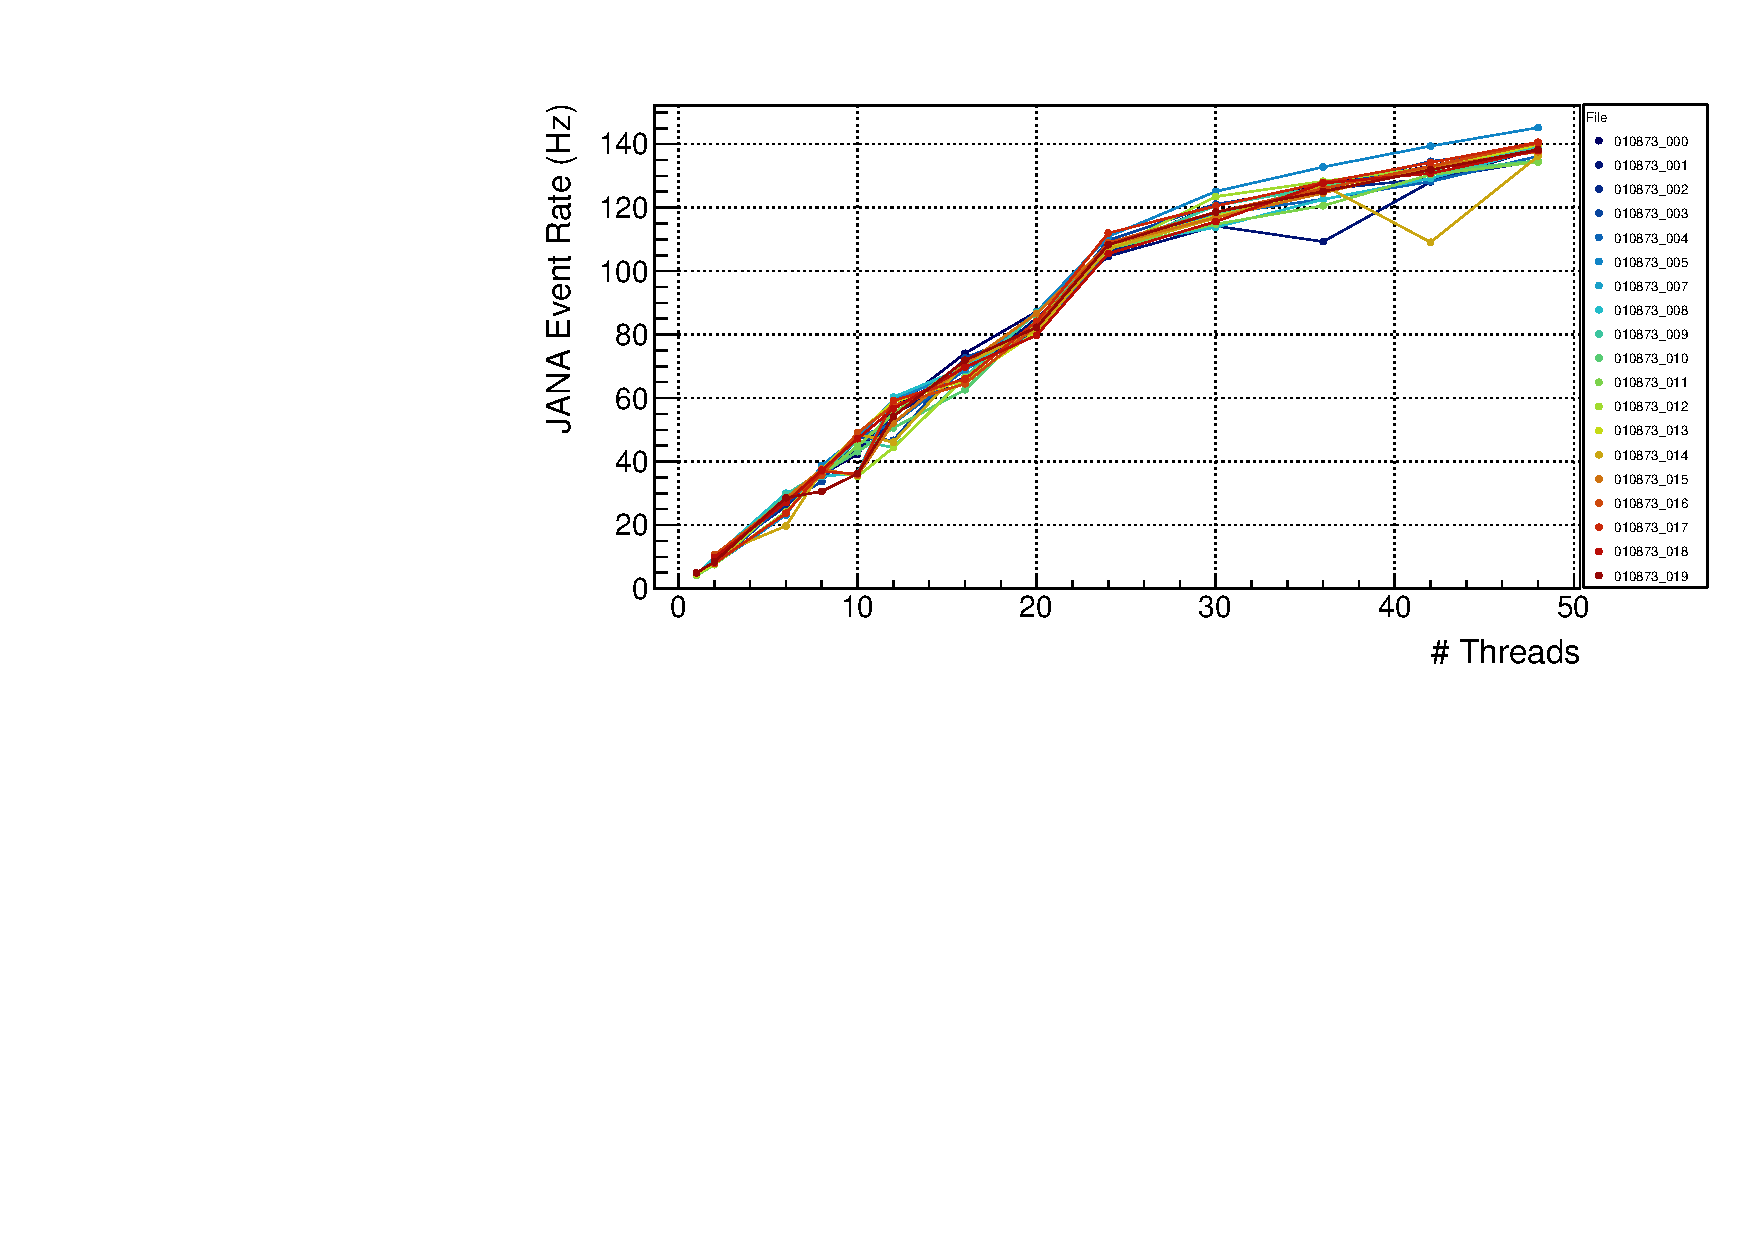
\includegraphics[width=0.7\textwidth]{figures/OfflineMonitor_PlotA.pdf}
\caption[]{\label{fig:offline_monitorA}The scaling of program performance as a function of
the number of processing threads.}
\end{figure}

The series of steps in the production of GlueX data will be describe in the following. In its initial phase, GlueX recorded about 1400 separate physics-quality runs with a unique run number, which have a total data footprint of about 3 petabytes. The data acquisition system saved the data in $19$ gigabyte files, with all runs consisting of multiple files (typically $100$ or more). Figure~\ref{fig:production_overview} shows an overview of the different production steps for GlueX data. 

\begin{figure}[h!]\centering
%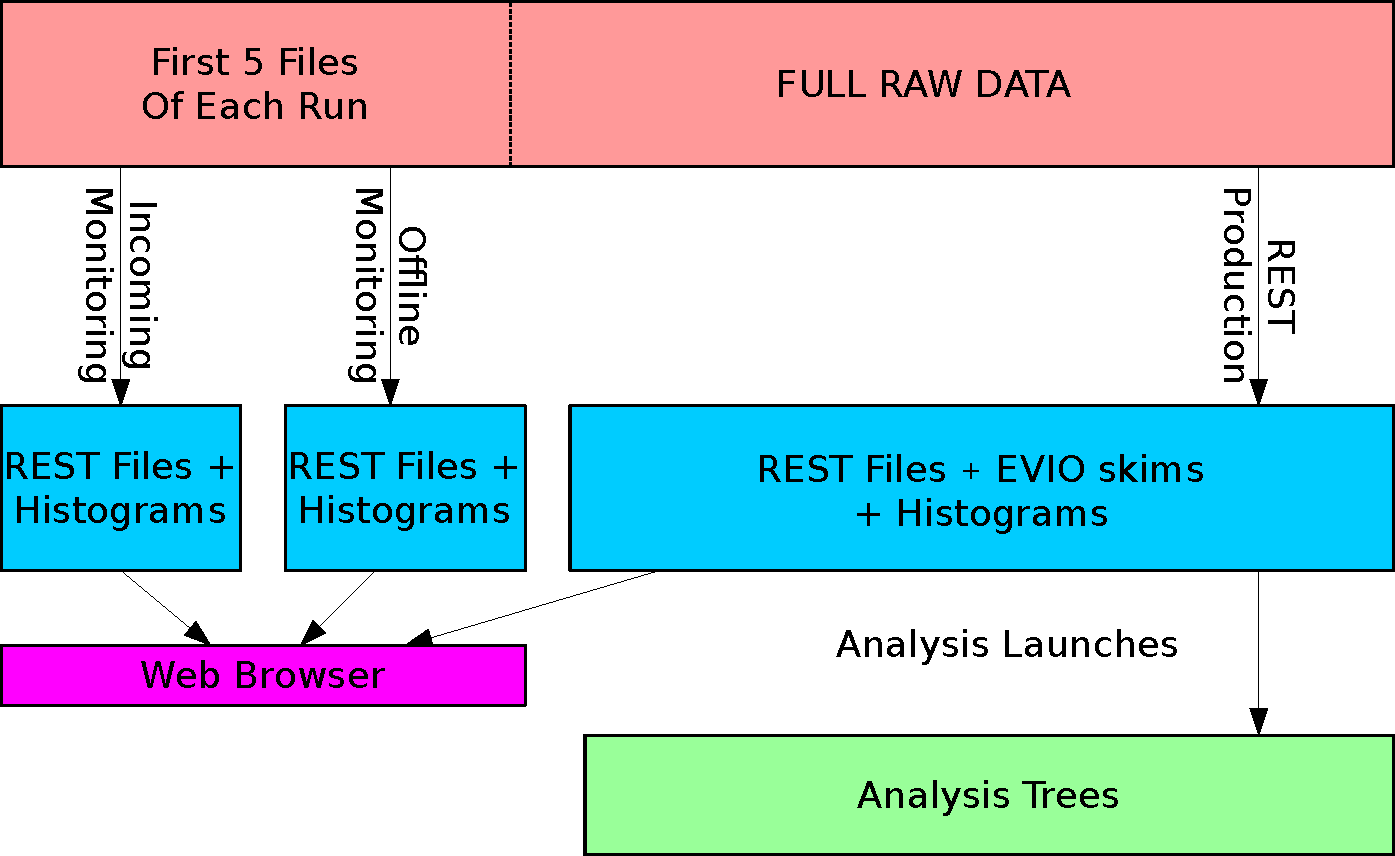
\includegraphics[width=0.8\textwidth]{figures/Production_generic.pdf}
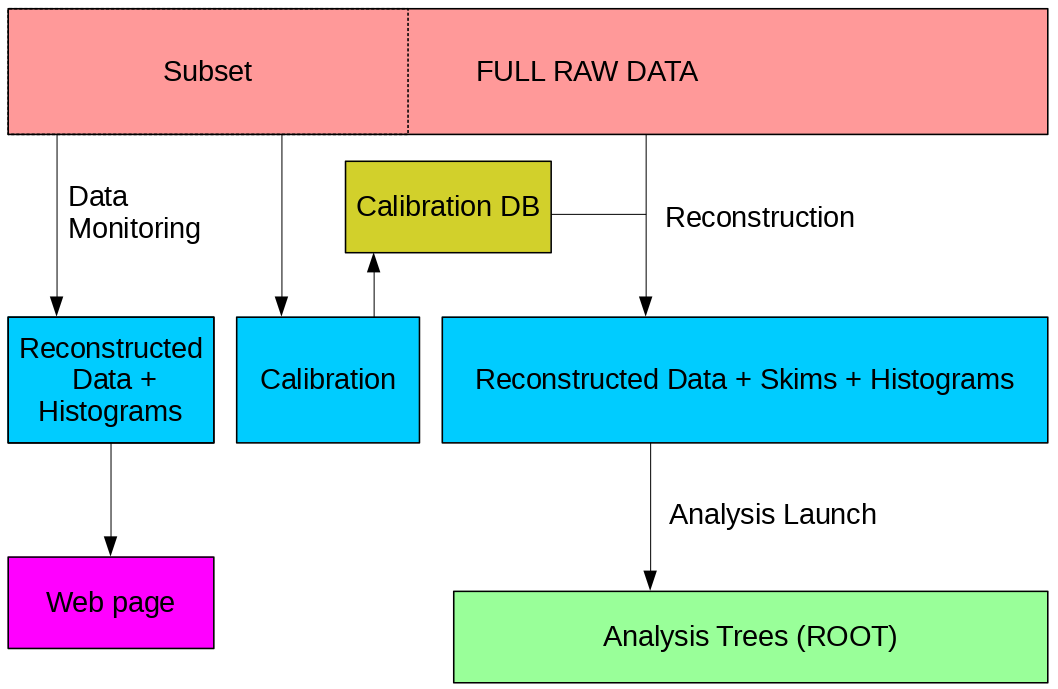
\includegraphics[width=0.8\textwidth]{figures/production_overview_calib.png}
\caption[]{\label{fig:production_overview}Production flow chart for GlueX data.} 
\end{figure}

\subsection{Calibration pass \label{sec:reccalibration}}

Two types of calibration jobs are running, depending on the complexity of the calibration procedures.  Simple, well-understood calibrations such as timing alignment between individual channels and subdetectors or drift chamber gain and time-to-distance calibrations, can be performed with one file of data per run.  These procedures are run either in the online environment or on the batch farm, and can be run several times as needed due to improvements in reconstruction algorithms or other calibrations.

More complicated calibration procedures, such as calorimeter gain calibration, require more data and are often iterative procedures, requiring several passes through the available data.  The raw data is processed on the batch farm as it comes into the computer center to produce the outputs needed for these procedures, either in the form of histograms or reduced skims in EVIO or ROOT tree format.  Many of these output require that charged particle tracks be reconstructed, but because of the computationally intensive nature of track reconstruction at GlueX, the available computing resources at JLab are insufficient for fully reconstructing all of the raw data as it comes in.  Therefore, only about $10-20$\% of the data has the full suite of calibration procedures applied.  The rest has a limited set of procedures, mostly focused on separating out events collected by specialized triggers. 
The individuals responsible for specific detector calibrations are then responsible for analyzing the skimmed data.

\subsection{Monitoring pass \label{sec:recmonitoring}}

The red-colored box at the top represents the experimental data that has been copied to the computer center. The small part of the box represents the first five files of each run, which are run through the offline monitoring processes. These monitoring jobs are first run during the run to check the quality of the data, but are also run after major changes to calibrations or software to validate those changes. These jobs produce both Reconstructed Events Storage (REST) files and root histogram files for checking the detector and reconstruction performance.

\subsection{Reconstruction pass \label{sec:recreconstruction}}

When the data is sufficiently well calibrated, we carry out a full production of the physics quality data. In the total GlueX data set, about 1400 of the runs were deemed physics quality. The remaining were short runs which were related to engineering and commissioning tests of the experiment. We note that while this number is small compared to the total number of runs, it is the vast majority of all data recorded during the running period, representing about 3 petabytes. All of these files are reconstructed and produce more than $500$ terabytes of REST data files. The large reduction is size from collected event data to physics data files allows us to  more quickly and efficiently carry out physics analyses on the data.
%, and is also small enough to be fully exported to off-site computer centers, see section~\ref{sec:remote-dist} (not really).

In the REST production, we included a series of detector performance studies that required access to raw data and would not be possible on the reconstructed data alone. Many improvements to software and detector calibration resulted from these studies. Similar studies can be made with simulated data to match and assess the detector acceptance.

\subsection{Offsite Reconstruction}
\label{sec:recoffsite}

\subsection{Analysis pass \label{sec:recanalysis}}

The full reconstructed (REST) data is too large to easily handled by individual analyzers. For that reason, we developed a system to centrally analyze data at Jefferson Lab to skim out final-state specific ROOT trees. This step is represented by the left-hand green box at the bottom of Figure~\ref{fig:production_overview}.

Users can submit individual reactions via a web interface (see Fig.~\ref{fig:production_analysis}). Periodically, the submitted reactions are downloaded into a configuration file, which steers the analysis launch. For each reaction, the GlueX analysis library inside the JANA framework creates possible particle combinations from the reconstructed charged tracks and showers saved in the REST format. Common selection criteria are applied for exclusivity and particle identification before performing a kinematic fit, using vertex and four-momentum constraints. Displaced vertices and inclusive reactions are also supported. Successful particle combinations (e.g. $\pi_0 \rightarrow \gamma\gamma$) and other objects are managed in memory pools and can be reused in between different channels to reduce the overall memory footprint of the process. With this scheme, we are able to bundle up to one hundred different reaction into one launch over the reconstructed data.

If the kinematic fit converged for one combination of tracks and showers, the event is stored into a reaction-specific but generic ROOT tree, made accessible to the whole collaboration. The total size of these ROOT trees for the full data set strongly depend on the selected reaction, but they are small enough to be copied to the user's home institution for a more detailed analysis.

\begin{figure}[h!]\centering
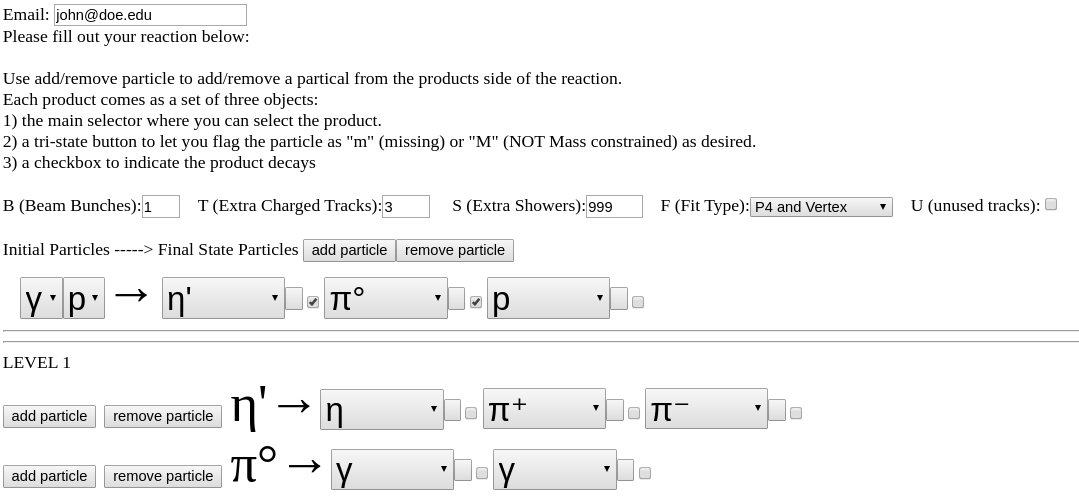
\includegraphics[width=\textwidth]{figures/analysis_submit_form.png}
\caption[]{\label{fig:production_analysis}Analysis submit form in browser.} 
\end{figure}